\testfile{pgfplotstest.file.tex}
{%
\lstset{
	showtabs=true,
	showspaces=true,
	basicstyle=\footnotesize\ttfamily,
	numbers=left,
	numberblanklines=true,
	breaklines=false,
	tabsize=10}

\testsection{`plot file' test}
\testsubsection{A file in gnuplot format 'num num i'}
\lstinputlisting{plotdata/pgfplotstest_plot2.gnuplot}
\begin{tikzpicture}
\begin{axis}
\addplot plot file{plotdata/pgfplotstest_plot2.gnuplot};
\end{axis}
\end{tikzpicture}

\testsubsubsection{Same file loaded with `plot table'}
\begin{tikzpicture}
\begin{axis}
\addplot plot table{plotdata/pgfplotstest_plot2.gnuplot};
\end{axis}
\end{tikzpicture}


\testsubsection{A file which differs slightly from gnuplot format}
\lstinputlisting{plotdata/pgfplotstest_plot4}
\begin{tikzpicture}
\begin{axis}
\addplot plot file{plotdata/pgfplotstest_plot4};
\end{axis}
\end{tikzpicture}

\testsubsection{A file which starts with newlines}
\lstinputlisting{plotdata/pgfplotstest_plot5}
\begin{tikzpicture}
\begin{axis}
\addplot plot file{plotdata/pgfplotstest_plot5};
\end{axis}
\end{tikzpicture}

\testsubsubsection{Same file loaded with `plot table'}
The first data point should have been identified as column name.

\begin{tikzpicture}
\begin{axis}
\addplot plot table{plotdata/pgfplotstest_plot5};
\end{axis}
\end{tikzpicture}

\testsubsubsection{Same file loaded with `plot table from macro'}
{
\pgfplotstableread{plotdata/pgfplotstest_plot5}\TABLEMACRO
\begin{tikzpicture}
\begin{axis}
\addplot plot table from \TABLEMACRO;
\end{axis}
\end{tikzpicture}
}

\testsubsubsection{testing space gobbling in `plot file' command}
\begin{tikzpicture}
\begin{axis}
\addplot plot file {plotdata/pgfplotstest_plot2.gnuplot};
\end{axis}
\end{tikzpicture}

\testsubsubsection{testing plot file `skip first' option to skip header}
\begin{tikzpicture}
	\begin{loglogaxis}[title=Read from file `pgfplotstest\_plot']
	\addplot file[skip first] {plotdata/pgfplotstest_plot};
	\end{loglogaxis}
\end{tikzpicture}

\testsection{`plot table' test}
\begin{sidewaystable}
\lstinputlisting{plotdata/pgfplotstest_plot}
\caption{\texttt{pgfplotstest\_plot}}
\end{sidewaystable}
\testsubsection{Plot by column `dof' versus column `Lmax'}
\begin{tikzpicture}
\begin{loglogaxis}[xlabel=Dof,ylabel=$L_\infty$ error,title=Read from file `pgfplotstest\_plot']
\addplot plot table[x=dof,y=Lmax] {plotdata/pgfplotstest_plot};
\end{loglogaxis}
\end{tikzpicture}


\testsubsection{Inline Data Format}
\testsubsubsection{Defaults}
\begin{tikzpicture}
	\begin{axis}
		\addplot table {
			col1 col2
			1 1
			2 2
			3 3
			4 4
			5 5
			6 6
		};
	\end{axis}
\end{tikzpicture}

\testsubsubsection{with scanline detection + different input selectors}
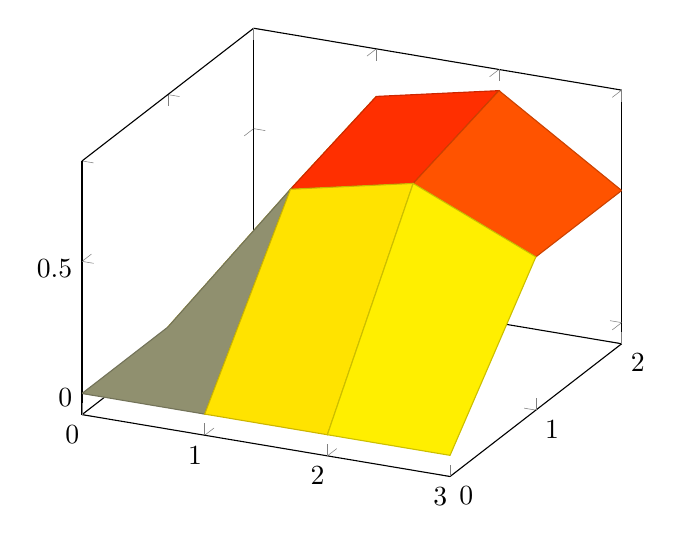
\begin{tikzpicture}
	\begin{axis}
		\addplot3[surf] table[y=col2,z expr=\thisrow{col3}*1] {
			col1 col2 col3
			 0 0 0
			 1 0 0
			 2 0 0
			 3 0 0 

			 0 1 0
			 1 1 0.6
			 2 1 0.7
			 3 1 0.5 

			 0 2 0
			 1 2 0.7
			 2 2 0.8
			 3 2 0.5 
		};
	\end{axis}
\end{tikzpicture}

\testsubsubsection{row sep=crcr}
\begin{tikzpicture}
	\begin{axis}
		\addplot table[row sep=crcr] {
			col1 col2\\
			1 1\\
			2 2\\
			3 3\\
			4 4\\
			5 5\\
			6 6\\
		};
	\end{axis}
\end{tikzpicture}

\testsubsubsection{row sep=crcr + macro arg}
{
	\def\content{
		\addplot table[row sep=crcr] {
			col1 col2\\
			1 1\\
			2 2\\
			3 3\\
			4 4\\
			5 5\\
			6 6\\
		};
	}
	\begin{tikzpicture}
		\begin{axis}
			\content
		\end{axis}
	\end{tikzpicture}
}
\testsubsubsection{row sep=crcr and col sep=ampersand}
\begin{tikzpicture}
	\begin{axis}
		\addplot table[col sep=&,row sep=\\] {
			col1 &col2\\
			1 &1\\
			2 &2\\
			3 &3\\
			4 &4\\
			5 &5\\
			6 &6\\
		};
	\end{axis}
\end{tikzpicture}

\testsubsubsection{row sep=crcr and col sep=ampersand}
\pgfplotstabletypeset[string type,col sep=&,row sep=\\]{
	col1 &col2\\
	1 &$1+1$\\
	2 &2\\
	3 &$3\cdot 4$\\
	4 &4\\
	5 &5\\
	6 &6\\
}

\pgfplotstabletypeset[columns/col1/.style={sci},columns/col2/.style={string type},col sep=&,row sep=\\]{
	col1 &col2\\
	1 &$1+1$\\
	2 &2\\
	3 &$3\cdot 4$\\
	4 &4\\
	5 &5\\
	6 &6\\
}

\testsubsubsection{row sep=crcr and scanline detection + different input selectors}
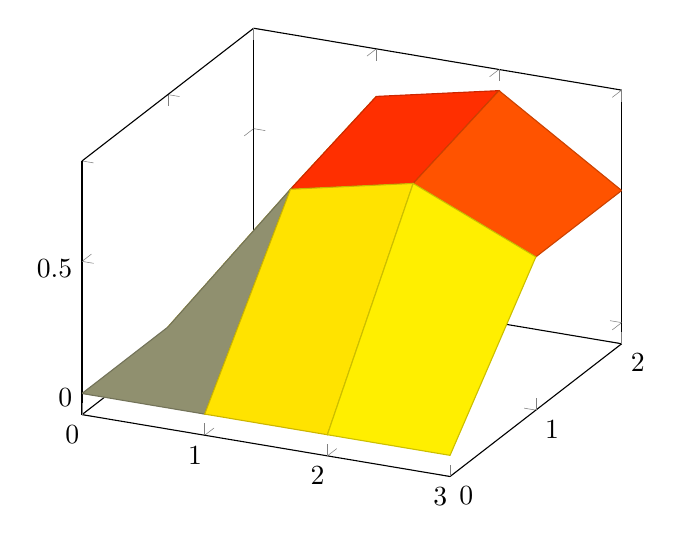
\begin{tikzpicture}
	\begin{axis}
		\addplot3[surf] table[y=col2,z expr=\thisrow{col3}*1,row sep=crcr] {
			col1 col2 col3\\
			 0 0 0\\
			 1 0 0\\
			 2 0 0\\
			 3 0 0 \\
\\
			 0 1 0\\
			 1 1 0.6\\
			 2 1 0.7\\
			 3 1 0.5 \\
\\
			 0 2 0\\
			 1 2 0.7\\
			 2 2 0.8\\
			 3 2 0.5 \\
		};
	\end{axis}
\end{tikzpicture}

{
\pgfplotstableset{
	alias/LmaxXX/.initial=Lmax,
	alias/{L/m=ax}/.initial=Lmax}
\testsubsection{Plot by column `dof' versus column `LmaxXX', a col alias}
\begin{tikzpicture}
\begin{loglogaxis}[xlabel=Dof,ylabel=$L_\infty$ error,title=Read from file `pgfplotstest\_plot']
\addplot plot table[x=dof,y=LmaxXX] {plotdata/pgfplotstest_plot};
\end{loglogaxis}
\end{tikzpicture}

\testsubsection{Plot by column `dof' versus column `L/m=ax', a col alias}
\begin{tikzpicture}
\begin{loglogaxis}[xlabel=Dof,ylabel=$L_\infty$ error,title=Read from file `pgfplotstest\_plot']
\addplot plot table[x=dof,y={L/m=ax}] {plotdata/pgfplotstest_plot};
\end{loglogaxis}
\end{tikzpicture}

\testsubsection{Plot by column `dof' versus column `L/m=ax', a col alias}
\begin{tikzpicture}
\begin{loglogaxis}[xlabel=Dof,ylabel=$L_\infty$ error,title=Read from file `pgfplotstest\_plot'; cdata using maxlevel]
\addplot+[scatter,point meta/expr=\thisrow{maxlevel}] plot table[x=dof,y={L/m=ax}] {plotdata/pgfplotstest_plot};
\end{loglogaxis}
\end{tikzpicture}

\testsubsection{Create on use}
\testsubsubsection{Typesetting the data with both, 'create on use' and col alias}
\pgfplotstabletypesetfile[
	create on use/order/.style={create col/dyadic refinement rate={L/m=ax}},
	columns={dof,L/m=ax,order},
]{plotdata/pgfplotstest_plot}

\testsubsubsection{Plotting data with col alias, scattersrc=ln(thisrow)}
\begin{tikzpicture}
	\begin{loglogaxis}[table/x=G,table/y={L/m=ax},]
	\addplot+[scatter,scatter src={ln(1e-8+\thisrow{L/m=ax})}] table {plotdata/pgfplotstest_plot};
	\end{loglogaxis}
\end{tikzpicture}

\testsubsubsection{Plotting data with 'create col/regression' feature}
\begin{tikzpicture}
\tracingmacros=2 \tracingcommands=2
	\begin{loglogaxis}[table/x=G,table/y={L/m=ax},]
	\addplot+[scatter,scatter src={ln(1e-8+\thisrow{L/m=ax})}] table {plotdata/pgfplotstest_plot};
	\addplot[red]
		table [y={create col/linear regression={y={L/m=ax},variance list={1000,1000,1000}}}]
		{plotdata/pgfplotstest_plot};
	\end{loglogaxis}
\end{tikzpicture}
}


\testsubsection{Plot by column \#2 versus column \#3}
\begin{tikzpicture}
\begin{loglogaxis}[
	xlabel=Dof,
	ylabel=$L_2$ error,
	title=Read from file `pgfplotstest\_plot'
]
\addplot plot table[x index=2,y index=3]{plotdata/pgfplotstest_plot};

\end{loglogaxis}
\end{tikzpicture}

\testsubsection{Plot by preloaded tables}
{
	\begin{sidewaystable}
		\lstinputlisting{plotdata/pgfplotstest_plot3}
		\caption{\texttt{pgfplotstest\_plot3}}
	\end{sidewaystable}
	\pgfnumtableread{plotdata/pgfplotstest_plot} to \tableA
	\pgfnumtableread{plotdata/pgfplotstest_plot3} to \tableB
	\begin{tikzpicture}
	\begin{loglogaxis}[
		xlabel=Dof,
		ylabel=$L_2$ error,
		title=Read from file `pgfplotstest\_plot' and `pgfplotstest\_plot3'
	]
		\addplot plot table[x=dof,y=L2] from \tableA;
		\addplot plot table[x=dof,y=L2] from \tableB;
		\legend{$d=2$\\$d=3$\\}%
	\end{loglogaxis}
	\end{tikzpicture}

	\testsubsubsection{Testing newline gobbling after optional args...}
	\pgfplotstabletypeset
		[sci,columns={dof,maxlevel}]
		\tableA

	\testsubsubsection{Testing newline gobbling in plot table}
	\begin{tikzpicture}
	\begin{loglogaxis}[
		xlabel=Dof,
		ylabel=$L_2$ error,
		title=Read from file `pgfplotstest\_plot'
	]
		\addplot table[x=dof,y=L2] 
			from 
			\tableA;
		\addplot table[x=dof,y=L2]
			{plotdata/pgfplotstest_plot};
		\legend{$d=2$\\$d=3$\\}%
	\end{loglogaxis}
	\end{tikzpicture}
}

\testsubsection{a table which has no column names}
\begin{sidewaystable}
\lstinputlisting{plotdata/pgfplotstest_plotnocolnames}
\caption{\texttt{plotdata/pgfplotstest\_plotnocolnames}}
\end{sidewaystable}
\begin{tikzpicture}
\begin{loglogaxis}[
	xlabel=Dof,
	ylabel=$L_2$ error,
	title=Read from file `pgfplotstest\_plotnocolnames'
]
\addplot plot table[x index=2,y index=3]{plotdata/pgfplotstest_plotnocolnames};

\end{loglogaxis}
\end{tikzpicture}

\clearpage
\testsection{Table Column Separators}


\long\def\testcolsep#1{%
	\lstinputlisting{plotdata/pgfplotstest_#1.dat}
	\pgfplotstabletypeset[col sep=#1]{plotdata/pgfplotstest_#1.dat}

	\begin{tikzpicture}
	\begin{axis}[
		title={col sep=#1.},
	]
	\addplot table[x=x,y=y,col sep=#1]{plotdata/pgfplotstest_#1.dat};

	\end{axis}
	\end{tikzpicture}
}
\testcolsep{comma}

\testcolsep{semicolon}

\testcolsep{colon}

\testcolsep{ampersand}

\testcolsep{braces}

	\lstinputlisting{plotdata/pgfplotstest_tab.dat}
	\pgfplotstabletypeset[col sep=tab]{plotdata/pgfplotstest_tab.dat}

	\begin{tikzpicture}
	\begin{axis}[
		title={col sep=tab.},
	]
	\addplot table[x=a long x name,y=y,col sep=tab]{plotdata/pgfplotstest_tab.dat};

	\end{axis}
	\end{tikzpicture}

\testsubsection{the same with active characters}
{
	\catcode`\;=13
	\def\testcolsep#1{%
		\begin{tikzpicture}
		\begin{axis}[
			title={col sep=#1.},
		]
		\addplot table[x=x,y=y,col sep=#1]{plotdata/pgfplotstest_#1.dat};

		\end{axis}
		\end{tikzpicture}
	}
	\testcolsep{semicolon}

	\catcode`\:=13
	\testcolsep{colon}
}

\testsection{`plot file' sanity checking test}
\testsubsection{2d}
\begin{tikzpicture}
	\begin{axis}[title=The input file has just one column.]
	\addplot file {plotdata/pgfplotstest_sanity.dat};
	\end{axis}
\end{tikzpicture}

\testsubsection{2d + meta}
\begin{tikzpicture}
	\begin{axis}[title=The input file has just one column.]
	\addplot+[scatter] file {plotdata/pgfplotstest_sanity.dat};
	\end{axis}
\end{tikzpicture}

\testsubsection{3d}
\begin{tikzpicture}
	\begin{axis}[title=The input file has just one column.]
	\addplot3 file {plotdata/pgfplotstest_sanity.dat};
	\end{axis}
\end{tikzpicture}

\testsubsection{3d + meta}
\begin{tikzpicture}
	\begin{axis}[title=The input file has just one column.]
	\addplot3+[scatter] file {plotdata/pgfplotstest_sanity.dat};
	\end{axis}
\end{tikzpicture}
}
